\section{Computer Engineering}

\begin{concept}{What is Computer Engineering?}\\
Computer Engineering is where microelectronics and software meet. It involves:
\begin{itemize}
  \item Architecture and organization of computer systems
  \item Combines hardware and software to implement a computer
  \item Applications in embedded systems, information technology, and technical/scientific tools
\end{itemize}
\end{concept}

\begin{definition}{Basic Hardware Components}\\
A computer system consists of four fundamental components:
\begin{itemize}
  \item \textbf{CPU (Central Processing Unit)}: Processes instructions and data
  \item \textbf{Memory}: Stores instructions and data
  \item \textbf{Input/Output}: Interface to external devices
  \item \textbf{System Bus}: Electrical connection between components
\end{itemize}

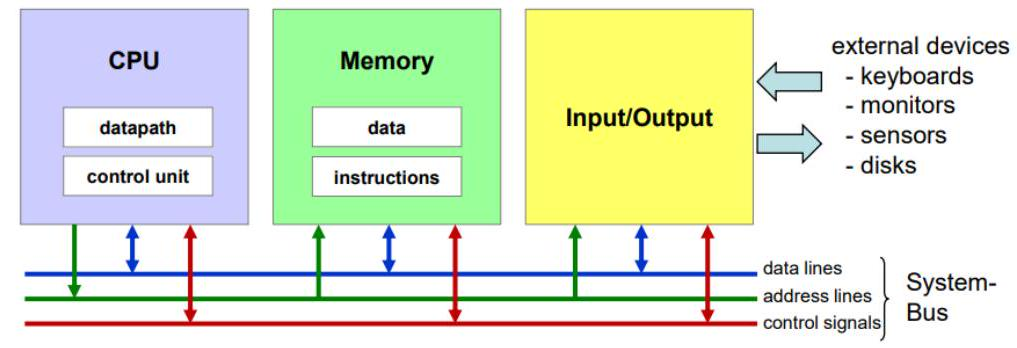
\includegraphics[width=\linewidth]{images/2024_12_29_79e6b22f503fb7b4f718g-01(1)}
\end{definition}

\begin{definition}{CPU Components}\\
The CPU contains several key components:
\begin{itemize}
  \item \textbf{Core Registers}: Fast but limited storage inside CPU
  \item \textbf{ALU (Arithmetic Logic Unit)}: Performs arithmetic and logic operations
  \item \textbf{Control Unit}: Reads and executes instructions
  \item \textbf{Bus Interface}: Connects CPU to system bus
\end{itemize}
\end{definition}

\begin{concept}{Memory Types}
\begin{itemize}
  \item \textbf{Main Memory (Arbeitsspeicher)}:
    \begin{itemize}
      \item Connected through System-Bus
      \item Access to individual bytes
      \item Volatile: SRAM, DRAM
      \item Non-volatile: ROM, Flash
    \end{itemize}
  \item \textbf{Secondary Storage}:
    \begin{itemize}
      \item Connected through I/O
      \item Access to blocks of data
      \item Non-volatile
      \item Examples: HDD, SSD, CD, DVD
    \end{itemize}
\end{itemize}
\end{concept}

\begin{formula}{Program Translation Process}\\
Translation from source code to executable involves four steps:

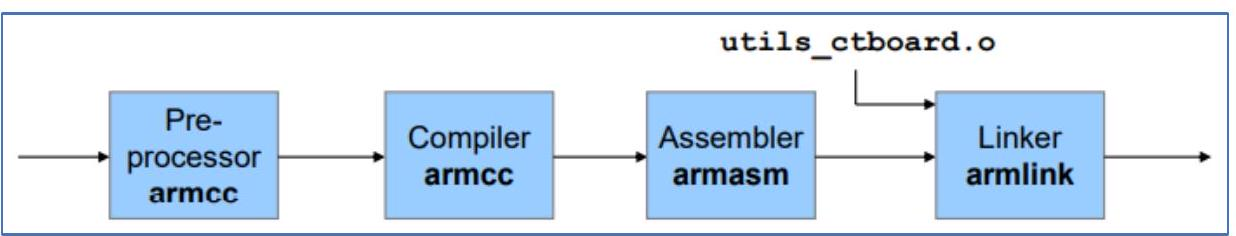
\includegraphics[width=\linewidth]{images/2024_12_29_79e6b22f503fb7b4f718g-01}

\begin{enumerate}
  \item \textbf{Preprocessor}:
    \begin{itemize}
      \item Text processing
      \item Includes header files
      \item Expands macros
      \item Output: Modified source program
    \end{itemize}
  \item \textbf{Compiler}:
    \begin{itemize}
      \item Translates C to assembly
      \item CPU-specific code generation
      \item Output: Assembly program
    \end{itemize}
  \item \textbf{Assembler}:
    \begin{itemize}
      \item Converts assembly to machine code
      \item Creates relocatable object file
      \item Output: Binary object file
    \end{itemize}
  \item \textbf{Linker}:
    \begin{itemize}
      \item Merges object files
      \item Resolves dependencies
      \item Creates executable program
      \item Output: Executable file
    \end{itemize}
\end{enumerate}
\end{formula}

\begin{KR}{Program Compilation Process}\\
To compile and link a program:
\begin{enumerate}
  \item Create source files (.c) and header files (.h)
  \item Run preprocessor to expand includes and macros
  \item Compile source files to object files
  \item Link object files and libraries
  \item Test executable
\end{enumerate}
\end{KR}

\begin{code}{Simple Program Translation - From Source to Executable}
\begin{lstlisting}[language=C, style=base]
#include <stdio.h>
#define MAX 100

int main(void) {
    printf("Max is %d\n", MAX);
    return 0;
}
\end{lstlisting}

Translation steps:
\begin{enumerate}
  \item Preprocessor expands include and replaces MAX with 100
  \item Compiler converts to assembly language
  \item Assembler creates object file
  \item Linker combines with C library to create executable
\end{enumerate}
\end{code}

\section{Computer Engineering}

\begin{concept}{What is Computer Engineering?}\\
Computer Engineering is where microelectronics and software meet. It involves:
\begin{itemize}
  \item Architecture and organization of computer systems
  \item Combines hardware and software to implement a computer
  \item Applications in embedded systems, information technology, and technical/scientific tools
  \item Historical development spanning over 70 years:
    \begin{itemize}
      \item 1940s: Relay/vacuum tubes
      \item 1950s: Transistors
      \item 1970s: Integrated circuits (CMOS)
      \item Present: Complex microprocessors with billions of transistors
    \end{itemize}
\end{itemize}
\end{concept}

\begin{example2}{Early Computing Milestones}\\
\begin{itemize}
  \item 1943: First electronic computer ENIAC (18,000 tubes, 30 tons, 140 kW)
  \item 1947: First transistor at Bell Labs
  \item 1971: First microprocessor Intel 4004 (2300 transistors)
  \item 1978: Intel 8086 (29,000 transistors)
  \item Modern processors: Over 5 billion transistors
\end{itemize}
\end{example2}

\begin{definition}{Basic Hardware Components}\\
A computer system consists of four fundamental components:
\begin{itemize}
  \item \textbf{CPU (Central Processing Unit)}: Processes instructions and data
  \item \textbf{Memory}: Stores instructions and data
  \item \textbf{Input/Output}: Interface to external devices
  \item \textbf{System Bus}: Electrical connection between components 
    \begin{itemize}
      \item Address lines: Select memory location
      \item Data lines: Transfer data (8/16/32/64 bits)
      \item Control signals: Coordinate operations
    \end{itemize}
\end{itemize}

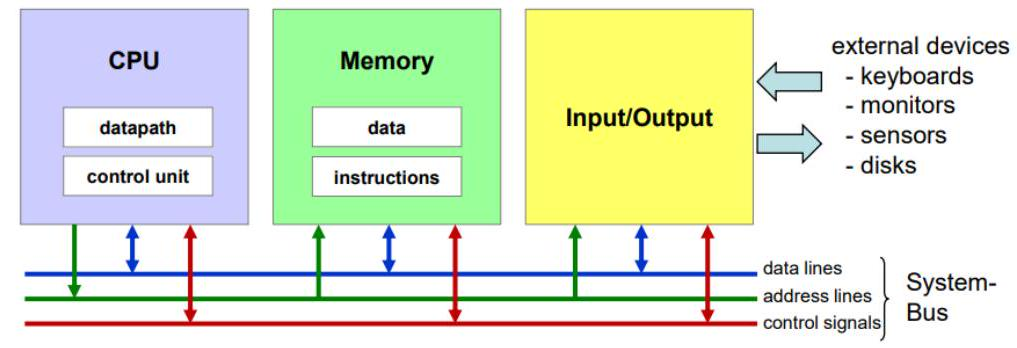
\includegraphics[width=\linewidth]{images/2024_12_29_79e6b22f503fb7b4f718g-01(1)}
\end{definition}

\begin{definition}{CPU Components}\\
The CPU contains several key components:
\begin{itemize}
  \item \textbf{Core Registers}: Fast but limited storage inside CPU
  \item \textbf{ALU (Arithmetic Logic Unit)}: Performs arithmetic and logic operations
  \item \textbf{Control Unit}: 
    \begin{itemize}
      \item Reads and executes instructions
      \item Controls program flow
      \item Manages instruction pipeline
    \end{itemize}
  \item \textbf{Bus Interface}: Connects CPU to system bus
\end{itemize}
\end{definition}

\begin{concept}{von Neumann Architecture}\\
The fundamental architecture used in most computers:
\begin{itemize}
  \item Single memory for both data and instructions
  \item Sequential instruction execution
  \item Components:
    \begin{itemize}
      \item Control unit
      \item ALU
      \item Memory
      \item Input/Output
    \end{itemize}
  \item Key limitation: Memory bottleneck ("von Neumann bottleneck")
\end{itemize}
\end{concept}

\begin{concept}{Memory Types}
\begin{itemize}
  \item \textbf{Main Memory (Arbeitsspeicher)}:
    \begin{itemize}
      \item Connected through System-Bus
      \item Access to individual bytes
      \item Volatile: 
        \begin{itemize}
          \item SRAM (Static RAM) - faster, more expensive
          \item DRAM (Dynamic RAM) - needs refresh, cheaper
        \end{itemize}
      \item Non-volatile: 
        \begin{itemize}
          \item ROM - factory programmed
          \item Flash - in-system programmable
        \end{itemize}
    \end{itemize}
  \item \textbf{Secondary Storage}:
    \begin{itemize}
      \item Connected through I/O
      \item Access to blocks of data
      \item Non-volatile
      \item Examples: HDD, SSD, CD, DVD
      \item Slower but cheaper than main memory
    \end{itemize}
\end{itemize}
\end{concept}

\begin{definition}{Memory Addressing}\\
\begin{itemize}
  \item Each byte in memory has a unique address
  \item Address space depends on address bus width:
    \begin{itemize}
      \item 8-bit address bus: 256 bytes ($2^8$)
      \item 16-bit address bus: 64 KB ($2^{16}$)
      \item 32-bit address bus: 4 GB ($2^{32}$)
    \end{itemize}
  \item Memory map shows allocation of address ranges
\end{itemize}
\end{definition}

\begin{formula}{Program Translation Process}\\
Translation from source code to executable involves four steps:

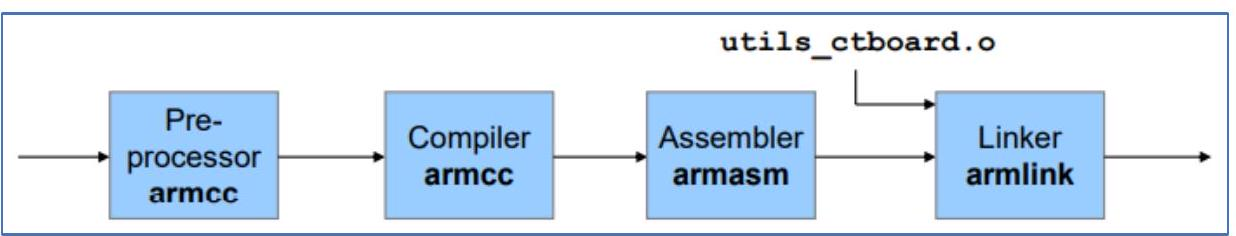
\includegraphics[width=\linewidth]{images/2024_12_29_79e6b22f503fb7b4f718g-01}

\begin{enumerate}
  \item \textbf{Preprocessor}:
    \begin{itemize}
      \item Text processing
      \item Includes header files (\#include)
      \item Expands macros (\#define)
      \item Output: Modified source program (.i)
    \end{itemize}
  \item \textbf{Compiler}:
    \begin{itemize}
      \item Translates C to assembly
      \item CPU-specific code generation
      \item Optimization (if enabled)
      \item Output: Assembly program (.s)
    \end{itemize}
  \item \textbf{Assembler}:
    \begin{itemize}
      \item Converts assembly to machine code
      \item Creates relocatable object file
      \item Generates symbol table
      \item Output: Binary object file (.o)
    \end{itemize}
  \item \textbf{Linker}:
    \begin{itemize}
      \item Merges object files
      \item Resolves dependencies
      \item Relocates addresses
      \item Links with libraries
      \item Output: Executable file (.axf)
    \end{itemize}
\end{enumerate}
\end{formula}

\begin{KR}{Program Compilation Process}\\
To compile and link a program:
\begin{enumerate}
  \item Create source files (.c) and header files (.h)
  \item Run preprocessor to expand includes and macros
  \item Compile source files to object files
  \item Link object files and libraries
  \item Test executable
\end{enumerate}

Common compiler flags:
\begin{itemize}
  \item -c: Compile only, don't link
  \item -o: Specify output file name
  \item -O[0-3]: Optimization level
  \item -g: Include debug information
\end{itemize}
\end{KR}

\begin{code}{Simple Program Translation - From Source to Executable}
\begin{lstlisting}[language=C, style=base]
// source.c
#include <stdio.h>
#define MAX 100

int main(void) {
    printf("Max is %d\n", MAX);
    return 0;
}
\end{lstlisting}

After preprocessing (.i):
\begin{lstlisting}[language=C, style=base]
// Contents of stdio.h included here
int main(void) {
    printf("Max is %d\n", 100);
    return 0;
}
\end{lstlisting}

Assembly output (.s):
\begin{lstlisting}[language=armasm, style=base]
    AREA |.text|, CODE, READONLY
    EXPORT main
main
    PUSH {LR}
    LDR R0, =string1
    LDR R1, =100
    BL printf
    MOVS R0, #0
    POP {PC}
    ALIGN
string1 DCB "Max is %d\n",0
    END
\end{lstlisting}
\end{code}

\begin{example2}{Host vs Target Development}\\
When developing for embedded systems:
\begin{itemize}
  \item \textbf{Host}: Development computer where code is written and compiled
  \item \textbf{Target}: Embedded system where code will run
  \item \textbf{Cross-compilation}: Compiling on host for different target architecture
  \item \textbf{Tool chain}: Complete set of development tools (compiler, linker, debugger)
\end{itemize}
\end{example2}

\begin{remark}
Understanding assembly language is important because it:
\begin{itemize}
  \item Helps understand machine-level operation
  \item Aids in debugging and optimization
  \item Required for system programming
  \item Essential for security analysis
\end{itemize}
\end{remark}